\chapter{Introduction}
\label{c:intro}

\newcommand{\ChapterRef}[1] {\Cref{#1}: \nameref{#1}}

\newcommand{\FourQueens}[2] {
  \begin{tikzpicture}[scale=0.6, every node/.style={black,scale=0.9}]
    \newcommand*{\xMin}{0}%
    \newcommand*{\xMax}{3}%
    \newcommand*{\yMin}{0}%
    \newcommand*{\yMax}{3}%
    \foreach \i / \label in {0/a,1/b,2/c,3/d} {
        \draw [] node at (\i+.5,\yMin-.3) {$\label$};
    }
    \foreach \i / \label in {0/1,1/2,2/3,3/4} {
        \draw [] node at (\xMin-.3,\i+.5) {$\label$};
    }

    \foreach \y in {0,2}{
        \foreach \x in {0,2}{
            \fill[black!8] (\x,\y) rectangle (1+\x,1+\y) rectangle (2+\x,2+\y);}}
    \draw [step=1.0] (0,0) grid (4,4);
    \foreach \x/\y/\m in {#2}
        \draw [] node at (\x,\y) {\m};
    \node[draw,circle,inner sep=1mm] at (-1.4,3.5) {#1};
  \end{tikzpicture}
}

\newcommand{\MCSDomains}[2] {
  \begin{tikzpicture}[scale=0.6, every node/.style={black,scale=0.9}]
    \newcommand*{\xMin}{0}%
    \newcommand*{\xMax}{5}%
    \newcommand*{\yMin}{0}%
    \newcommand*{\yMax}{4}%
    \foreach \i / \label in {0/a,1/b,2/c,3/d,4/e,5/f} {
        \draw [] node at (\i+.5,\yMax+1.4) {$\label$};
    }
    \foreach \i / \label in {4/1,3/2,2/3,1/4,0/5} {
        \draw [] node at (\xMin-.3,\i+.5) {$\label$};
    }

    \draw [step=1.0] (0,0) grid (6,5);
    \foreach \x/\y/\m in {#2}
        \draw [] node at (\x,\y) {\m};
    \node[draw,circle,inner sep=1mm] at (-1.4,3.5) {#1};
  \end{tikzpicture}
}

Graphs --- collections of items (vertices), some pairs of which
are related --- can be used to model
systems from a huge variety of domains.  A molecule can be viewed as a collection
of vertices (the atoms) joined together by bonds
\citep{sussenguth1965graph}; 
an image may be summarised using a vertex for each coloured region
with adjacent vertices joined \citep{DBLP:conf/icip/OlatunbosunDE96}.
We may wish to determine whether all or a large
part of a given object --- such as a molecule or image --- is contained
in another given object.  This dissertation presents new algorithms
for such problems.

The first problem we consider is the \emph{maximum common induced subgraph}
family of problems: we seek to find a large subgraph that is
contained in each of two given graphs.
Depending on the flavour of the problem, these
graphs may be directed or undirected and may or may not have labels.
All of these variants of the can be handled by the \McSplit\ family of algorithms.
These algorithms use a simple, fast and space-efficient data structure to keep
track of the set of vertices in the second graph to which a given vertex
in the first graph may be mapped.

The second problem we consider is \emph{induced subgraph isomorphism}: to determine
whether a given graph (the ``target graph'') contains another given graph (the ``pattern graph'')
as an induced subgraph.  We again use a variant of the \McSplit\ algorithm ---
\McSplit-SI --- to solve the problem; this version of the algorithm has a specialised
version of \McSplit's data structure that allows very fast processing of sparse graphs.

For the final problem considered in this dissertation, we turn from subgraphs
to supergraphs.  We study the problem of finding, for a given family of graphs,
an \textit{induced universal graph} --- that is, a graph that contains every
member of the family as an induced subgraph --- with as few vertices as
possible.  This problem generalises the \textit{minimum common supergraph}
problem to an arbitrary number of input graphs.  Although much progress has
been made on asymptotic results on the size of induced universal graphs, almost no
work has been done on developing algorithms to solve the problem exactly.  This
dissertation presents an algorithm for finding minimal induced universal graphs
using \McSplit-SI as a subroutine, and presents new terms of integer sequences
generated using the program.  Further, we present a hill-climbing method for
finding small (although possibly not optimal) induced universal graphs.

\section{Preliminaries}

A graph $G$ is a pair $(V, E)$ whose \emph{vertex set} $V = V(G)$
is an arbitrary finite set and whose \emph{edge set} $E = E(G)$
comprises two-elements subset of $V$. The elements of each edge
$e \in E$ are called its \emph{endpoints}, and two vertices that
are the endpoints of some edge are said to be \emph{adjacent}.

For example, \Cref{fig:g1} shows the graph $G_1 = (V,E)$, where
\[
V = \{1, 2, 3, 4, 5, 6\},
E = \{\{1,2\}, \{1,3\}, \{2,3\}, \{3,4\}, \{4,5\}, \{4,6\}, \{5,6\}\}
.
\]

\begin{figure}[htb]
    \centering
    \subfigure[][$G_1$] {
        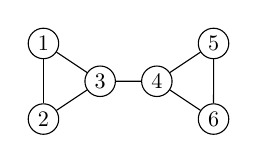
\begin{tikzpicture}[scale=0.6, every node/.style={scale=0.8,inner sep=.7mm}]
          \node [draw,circle] (1) at (0,1.6) {1};
          \node [draw,circle] (2) at (0,0) {2};
          \node [draw,circle] (3) at (1.2,.8) {3};
          \node [draw,circle] (4) at (2.4,.8) {4};
          \node [draw,circle] (5) at (3.6,1.6) {5};
          \node [draw,circle] (6) at (3.6,0) {6};
          \draw (1) -- (2);
          \draw (1) -- (3);
          \draw (2) -- (3);
          \draw (3) -- (4);
          \draw (4) -- (5);
          \draw (4) -- (6);
          \draw (5) -- (6);
        \end{tikzpicture}
        \label{fig:g1}
    }
    \quad\subfigure[][$G_2$] {
        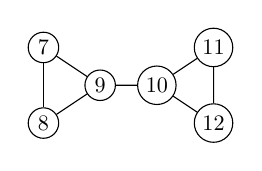
\begin{tikzpicture}[scale=0.6, every node/.style={scale=0.8,inner sep=.7mm}]
          \node [draw,circle] (1) at (0,1.6) {7};
          \node [draw,circle] (2) at (0,0) {8};
          \node [draw,circle] (3) at (1.2,.8) {9};
          \node [draw,circle] (4) at (2.4,.8) {10};
          \node [draw,circle] (5) at (3.6,1.6) {11};
          \node [draw,circle] (6) at (3.6,0) {12};
          \draw (1) -- (2);
          \draw (1) -- (3);
          \draw (2) -- (3);
          \draw (3) -- (4);
          \draw (4) -- (5);
          \draw (4) -- (6);
          \draw (5) -- (6);
        \end{tikzpicture}
        \label{fig:g2}
    }
    \quad\subfigure[][$G_3$] {
        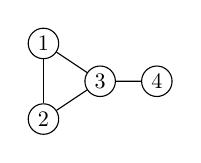
\begin{tikzpicture}[scale=0.6, every node/.style={scale=0.8,inner sep=.7mm}]
          \node [draw,circle] (1) at (0,1.6) {1};
          \node [draw,circle] (2) at (0,0) {2};
          \node [draw,circle] (3) at (1.2,.8) {3};
          \node [draw,circle] (4) at (2.4,.8) {4};
          \draw (1) -- (2);
          \draw (1) -- (3);
          \draw (2) -- (3);
          \draw (3) -- (4);
        \end{tikzpicture}
        \label{fig:g3}
    }
%    \quad\subfigure[][$G_4$] {
%        \begin{tikzpicture}[scale=0.6, every node/.style={scale=0.8,inner sep=.7mm}]
%          \node [draw,circle] (1) at (0,1.6) {1};
%          \node [draw,circle] (2) at (0,0) {2};
%          \node [draw,circle] (3) at (1.2,.8) {3};
%          \node [draw,circle] (4) at (2.4,1.6) {4};
%          \node [draw,circle] (5) at (2.4,0) {5};
%          \draw (1) -- (2);
%          \draw (1) -- (3);
%          \draw (2) -- (3);
%          \draw (3) -- (4);
%          \draw (3) -- (5);
%          \draw (4) -- (5);
%        \end{tikzpicture}
%        \label{fig:g4}
%    }
    \caption{Example graphs $G_1$ to $G_3$}
    \label{fig:intro-examples}
\end{figure}

A \emph{loop} is an edge from a vertex to itself. We assume throughout this
dissertation that graphs have no loops, except in clearly marked sections where
we discuss extensions of algorithms to graphs with loops.

The set of vertices adjacent to vertex $v \in V(G)$
is called the \emph{neighbourhood} of $v$, denoted $\N_G(v)$. We denote
by $\invN_G(v)$ the \emph{inverse neighbourhood} of $v$: the set
of the vertices other than $v$ itself that are not adjacent to $v$.
We omit the subscript $G$ where there is no ambiguity.
In \Cref{fig:g1}, for example, we have $\N(3) = \{1,2,4\}$ and
$\invN(3) = \{5,6\}$.

We say that graphs $G$ and $H$ are \emph{isomorphic} if we can relabel
the vertices of $G$ to produce graph $H$. For example, graphs $G_1$
and $G_2$ in \Cref{fig:intro-examples} are isomorphic.
Formally, an isomorphism between graphs $G$ and $H$ is a bijection $f$
from $V(G)$ to $V(H)$, such that $E(H) = \{\{f(u), f(v)\} \mid \{u, v\} \in E(G)\}$.
If such an $f$ exists, we say that $G$ and $H$ are isomorphic.

The \emph{line graph} of a graph $G=(V,E)$ is a graph with a vertex for each element
of $E$, such that two vertices are adjacent if and only if their corresponding edges
in $G$ share an endpoint.

An \emph{induced subgraph} of $G = (V, E)$ has a subset $W \subseteq V$ as its
vertex set, and $\{\{u, v\} \in E \mid \{u, v\} \in W\}$ as its edge set; that
is, the subgraph includes all edges of $G$ whose endpoints both appear in
$W$.  We say that this subgraph is \emph{induced by} $W$.
Graph $G_3$ of \Cref{fig:intro-examples} is thus the subgraph
of $G_1$ induced by the set $\{1,2,3,4\}$.
A \emph{subgraph} (without the ``induced'' qualifier) is an induced subgraph
with zero or more of the edges deleted.

A \emph{common induced subgraph} of graphs $G$ and $H$ is an induced subgraph
of $G$ which is isomorphic to an induced subgraph of $H$. In
\Cref{fig:cis-example}, a common induced subgraph of the two graphs (which is
induced by $\{1,2,3,4\}$) is highlighted on the first graph, and its isomorphic
subgraph is highlighted on the second graph.  It is often convenient to summarise
a common induced subgraph and its associated isomorphism $f$ by the \emph{mapping}
$\{(v,f(v)) \mid v \in W\}$, where $W \subseteq V$ is the set of vertices that
induces the common subgraph.  In our example, $M = \{(1,6), (2,7), (3,8), (4,9)\}$.

\begin{figure}[h!]
\centering
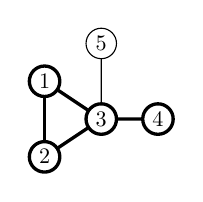
\begin{tikzpicture}[scale=0.6, every node/.style={scale=0.8,inner sep=.7mm}]
  \node [very thick,draw,circle] (1) at (0,1.6) {1};
  \node [very thick,draw,circle] (2) at (0,0) {2};
  \node [very thick,draw,circle] (3) at (1.2,.8) {3};
  \node [very thick,draw,circle] (4) at (2.4,.8) {4};
  \node [draw,circle] (5) at (1.2,2.4) {5};
  \draw [very thick] (1) -- (2);
  \draw [very thick] (1) -- (3);
  \draw [very thick] (2) -- (3);
  \draw [very thick] (3) -- (4);
  \draw (3) -- (5);
\end{tikzpicture}
\qquad
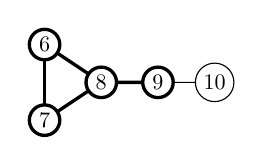
\begin{tikzpicture}[scale=0.6, every node/.style={scale=0.8,inner sep=.7mm}]
  \node [very thick,draw,circle] (1) at (0,1.6) {6};
  \node [very thick,draw,circle] (2) at (0,0) {7};
  \node [very thick,draw,circle] (3) at (1.2,.8) {8};
  \node [very thick,draw,circle] (4) at (2.4,.8) {9};
  \node [draw,circle] (5) at (3.6,.8) {10};
  \draw [very thick] (1) -- (2);
  \draw [very thick] (1) -- (3);
  \draw [very thick] (2) -- (3);
  \draw [very thick] (3) -- (4);
  \draw (4) -- (5);
\end{tikzpicture}
\caption{A pair of graphs with a maximum common induced subgraph highlighted}
\label{fig:cis-example}
\end{figure}

A \emph{maximum common induced subgraph (MCIS)} of $G$ and $H$ is a common
induced subgraph of $G$ and $H$ whose vertex set is as large as possible; the
common induced subgraph in \Cref{fig:cis-example} is an example of an MCIS.

A \emph{clique} is a set of vertices that are mutually adjacent, and the
\emph{maximum clique problem} is, given a graph $G$, to find a clique in $G$
with as many vertices as possible.

A \emph{labelled graph} (or \emph{network}) is a triple $(G, f_v, f_e)$
where $G$ is a graph,
the \emph{vertex label function} $f_v$ is a function with domain $V(G)$,
and the \emph{edge label function} $f_e$ is a function with domain $E(G)$.
The maximum common induced subgraph problem has a natural extension to labelled graphs
where we require the isomorphism to preserve labels on vertices and edges.

A \emph{directed graph} is a pair $(V,A)$, where $V$ is the vertex set and $A$,
a set of ordered pairs of elements of $V$, is the arc set.  The definitions of
\emph{induced subgraph}, \emph{isomorphism} and \emph{maximum common induced
subgraph} for directed graphs are analogous to their counterparts for graphs.
\label{fig:directed-cis-example} shows two directed graphs with a common
induced subgraph highlighted.

\begin{figure}[h!]
\centering
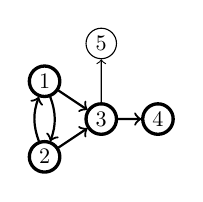
\begin{tikzpicture}[scale=0.6, every node/.style={scale=0.8,inner sep=.7mm}]
  \node [very thick,draw,circle] (1) at (0,1.6) {1};
  \node [very thick,draw,circle] (2) at (0,0) {2};
  \node [very thick,draw,circle] (3) at (1.2,.8) {3};
  \node [very thick,draw,circle] (4) at (2.4,.8) {4};
  \node [draw,circle] (5) at (1.2,2.4) {5};
  \draw [->,thick,bend left=20] (1) edge (2);
  \draw [->,thick,bend left=20] (2) edge (1);
  \draw [->,thick] (1) edge (3);
  \draw [->,thick] (2) edge (3);
  \draw [->,thick] (3) edge (4);
  \draw [->] (3) edge (5);
\end{tikzpicture}
\qquad
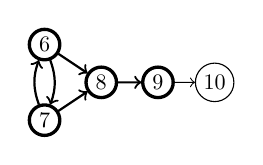
\begin{tikzpicture}[scale=0.6, every node/.style={scale=0.8,inner sep=.7mm}]
  \node [very thick,draw,circle] (1) at (0,1.6) {6};
  \node [very thick,draw,circle] (2) at (0,0) {7};
  \node [very thick,draw,circle] (3) at (1.2,.8) {8};
  \node [very thick,draw,circle] (4) at (2.4,.8) {9};
  \node [draw,circle] (5) at (3.6,.8) {10};
  \draw [->,thick,bend left=20] (1) edge (2);
  \draw [->,thick,bend left=20] (2) edge (1);
  \draw [->,thick] (1) edge (3);
  \draw [->,thick] (2) edge (3);
  \draw [->,thick] (3) edge (4);
  \draw [->] (4) edge (5);
\end{tikzpicture}
\caption{A pair of directed graphs with a maximum common induced subgraph highlighted}
\label{fig:directed-cis-example}
\end{figure}

For arc $(u,v)$, we say that $u$ is the source vertex and $v$ is target vertex; both
$u$ and $v$ are called endpoints.

\section{Problems covered by this dissertation}

This dissertation presents algorithms for the following three problems.

\begin{itemize}
    \item \textbf{Maximum common induced subgraph.} Find
a maximum common induced subgraph of two given graphs.
    \item \textbf{Induced subgraph isomorphism.} Given graphs $G$ and $H$,
determine whether $G$ is isomorphic to an induced subgraph of $H$;
if so, return the isomorphism.
    \item \textbf{Minimum induced universal graph.} Given a family of graphs $\calF$,
find a graph with as few vertices as possible that contains each member of $\calF$
as an induced subgraph.
\end{itemize}

Each of the three problems can be seen to be NP-hard by a simple reduction from \textsc{Clique}.
Given graph $G$ and natural number $k$, we can determine whether $G$ contains a clique
of size $k$ by solving either of the first two problems with the complete graph $K_k$ as
the first graph and $G$ as the second, or by solving the third problem with the family
$\{K_k, G\}$ as input.

\section{Related Problems}

This section briefly introduces three problems that are closely related to
maximum common induced subgraph and induced subgraph isomorphism.

The \emph{graph isomorphism problem} is a special case of the induced subgraph
isomorphism problem in which the two input graphs have the same number of
vertices.  Most state of the art algorithms for graph isomorphism, such as
Nauty and Traces, solve the problem by computing a canonical representation of
each graph and comparing these representations \citep{McKay201494}.  The
canonical representations may then be re-used for comparisons with other
graphs.  Considering only pairwise comparisons of graphs, a 2001 study found
that the induced subgraph isomorphism solver VF2 outperformed Nauty on several
classes of graph \citep{foggia2001performance}.  While we do not consider graph
isomorphism further in this dissertation, it would be an interesting topic of
future work to test whether the current state of the art subgraph isomorphism
solvers outperform the best graph isomorphism solvers on some interesting
classes of graphs.

Induced subgraph isomorphism and maximum common induced subgraph each have a
non-induced counterpart. The \emph{subgraph monomorphism problem} is to determine
whether graph $G$ is isomorphic to a subgraph of graph $H$, without the requirement
that the subgraph be induced.
This problem is also known as \emph{subgraph isomorphism} (without
the ``induced'' qualifier), but we will use the name subgraph monomorphism
to avoid confusion with induced subgraph isomorphism.

The \emph{maximum common edge subgraph (MCES)} problem is to find a subgraph of
graph $G$ with as many edges as possible that is isomorphic to a subgraph of
graph $H$, again without requiring the subgraphs to be induced.
There is a close connection between this problem and MCIS: by a
result due to \citet{whitney1932congruent}, we can find the MCES two
graphs by searching for an MCIS on their line graphs.  This approach has a
small complication: the triangle graph $K_3$ and the claw graph $K_{1,3}$
(\cref{fig:k3-and-claw}) both have $K_3$ as their line graph, and we must
therefore check during search that a triangle in $G$ is not mapped to a claw
in $H$ or vice versa.

\begin{figure}[htb]
    \centering
    \begin{tikzpicture}[scale=.35, every node/.style={black,scale=0.7}]%{{{
    \node[draw, circle, fill=white, inner sep=1.4pt, font=\bfseries] (Na) at (1,  0)
    {\vphantom{0}};
    \node[draw, circle, fill=white, inner sep=1.4pt, font=\bfseries] (Nb) at (0, -2)
    {\vphantom{0}};
    \node[draw, circle, fill=white, inner sep=1.4pt, font=\bfseries] (Nc) at (2, -2)
    {\vphantom{0}};

    \draw [edge] (Na) -- (Nb);
    \draw [edge] (Nb) -- (Nc);
    \draw [edge] (Na) -- (Nc);

\end{tikzpicture}
\qquad
\begin{tikzpicture}[scale=.35, every node/.style={black,scale=0.7}]%{{{
    \node[draw, circle, fill=white, inner sep=1.4pt, font=\bfseries] (Na) at (-.2,  -.2)
    {\vphantom{0}};
    \node[draw, circle, fill=white, inner sep=1.4pt, font=\bfseries] (Nb) at (2.2, -.2)
    {\vphantom{0}};
    \node[draw, circle, fill=white, inner sep=1.4pt, font=\bfseries] (Nc) at (1, -1.5)
    {\vphantom{0}};
    \node[draw, circle, fill=white, inner sep=1.4pt, font=\bfseries] (Nd) at (1, -3)
    {\vphantom{0}};

    \draw [edge] (Na) -- (Nc);
    \draw [edge] (Nb) -- (Nc);
    \draw [edge] (Nc) -- (Nd);

\end{tikzpicture}

    \caption{The graphs $K_3$ and $K_{1,3}$.}
    \label{fig:k3-and-claw}
\end{figure}

Several algorithms for MCES, such as RASCAL
\citep{DBLP:journals/cj/RaymondGW02}, use this method, as we will discuss further
in the next section.  \citet{DBLP:conf/mco/VismaraV08} describe how this technique
can be used on labelled graphs.

The present author's preliminary work on using the \McSplit\ algorithm
described in this thesis for MCES shows promising results
\citep{trimble2018three}. This would be a useful direction for future work, but
it is not pursued further in this dissertation.

%The maximum clique problem is to find an induced subgraph of a graph $G$ with as
%many vertices as possible, such that the subgraph has all possible edges; that
%is ??. Maximum clique can be solved (although rather inefficiently in practice)
%using an MCIS algorithm, by finding the MCIS of $G$ and a complete graph with the
%same number of vertices as $G$.

\section{Constraint Programming}

A \emph{constraint satisfaction problem (CSP)} is a problem of finding a value
for each of a finite set of variables, subject to a set of constraints.
This framework is extremely broad, and has applications in fields
including logistics, scheduling, bioinformatics, and discrete mathematics.
The field of \emph{constraint programming} is concerned with modelling
and solving constraint satisfaction problems. Many algorithms in the literature
for MCIS and induced subgraph isomorphism model these problems as CSPs.
Moreover, the \McSplit\ family of algorithms introduced in this dissertation
are closely related to a constraint programming approach.
This section gives a brief introduction to constraint programming;
a detailed treatment can be found in the \emph{Handbook of Constraint
Programming} \citep{DBLP:reference/fai/2}.

Formally, a CSP is a triple $\langle X, D, C\rangle$, where

\begin{itemize}
\item $X$ is a tuple of \emph{variables} $X = \langle x_1, x_2, \dots, x_n \rangle$,
\item $D$ is a corresponding tuple of finite \emph{domains} $D = \langle D_1, D_2, \dots, D_n\rangle$
  such that each $x_i$ must take a value in $D_i$,
\item $C$ is a tuple of constraints, each of which acts on a subset of $X$ and restricts
  the values that may be taken simulatenously by those variables.
\end{itemize}

A solution to a CSP is an assignment of domain values to each variable in $X$
satisfying the constraints $C$.

Broadly, algorithms for solving CSPs can be classed as \emph{complete} (guaranteed to find a solution)
or \emph{incomplete}. The former category is the focus of this dissertation.
Complete algorithms---which are the focus of our dissertation---may further
be subdivided into backtracking search algorithms and dynamic programming
algorithms. All of the constraint programming approaches to MCIS and induced
subgraph isomorphism use some form of backtracking search, and therefore that will
be the focus of this chapter.

To illustrate the process of solving a CSP, we use a canonical introductory
problem, $n$-queens. For our example, we will consider the case $n=4$. The problem
is to place four queens on a $4 \times 4$ chessboard such that no two queens
are in the same row, column, or diagonal.

The first step is to model the problem as a CSP. Many models have been proposed
for the $n$-queens problem \citep{DBLP:reference/fai/Smith06}; we will use a
simple model with one variable per row ($x_1$ to $x_4$) and four values, $\{a, b, c, d\}$, for
the four columns.  There are two types of constraint. First, there is a single
\emph{allDifferent} constraint ensuring the four variables take different
values (and thus the queens are in different columns). Second, there is a
constraint for each of the ten diagonals that have more than one square
ensuring that at most one queen is placed on that diagonal.

\Cref{fig:FourQueens} shows a search tree for this problem. At node A,
no assignments of values to variables have been made. At node B, a first
tentative assignment has been made: $x_1=a$. A key part of most backtracking CP
solvers is the interleaving of search (trying possible values for a variable
in turn) with \emph{constraint propagation} (deleting values that can be
determined not to appear in any solution that extends the current set of
assignments). For our example, we will use the simplest form of propagation:
emph{forward checking}. This removes from the domains of the unassigned variables
every value that conflicts with some existing assignment. The $\times$ symbol
in a square in the figure indicates that a value has been removed from a domain.

At node C, the assignment $x_2=c$ has been made. After forward checking, no
values are left in $D_3$; thus there is no solution with $x_1=a$ and $x_2=c$.
The algorithm backtracks and tries $x_2=d$
(node D). This process of search, forward checking, and backtracking when
a domain becomes empty is continued (nodes E to I) until reaching the solution
shown in node I.

\newsavebox{\FourQueensBoxA}
\newsavebox{\FourQueensBoxB}
\newsavebox{\FourQueensBoxC}
\newsavebox{\FourQueensBoxD}
\newsavebox{\FourQueensBoxE}
\newsavebox{\FourQueensBoxF}
\newsavebox{\FourQueensBoxG}
\newsavebox{\FourQueensBoxH}
\newsavebox{\FourQueensBoxI}
\sbox{\FourQueensBoxA}{\FourQueens{A}{0.5/0.5/,1.5/0.5/,2.5/0.5/,3.5/0.5/,0.5/1.5/,1.5/1.5/,2.5/1.5/,3.5/1.5/,0.5/2.5/,1.5/2.5/,2.5/2.5/,3.5/2.5/,0.5/3.5/,1.5/3.5/,2.5/3.5/,3.5/3.5/}}
\sbox{\FourQueensBoxB}{\FourQueens{B}{0.5/0.5/\symqueen,1.5/0.5/$\times$,2.5/0.5/$\times$,3.5/0.5/$\times$,0.5/1.5/$\times$,1.5/1.5/$\times$,2.5/1.5/,3.5/1.5/,0.5/2.5/$\times$,1.5/2.5/,2.5/2.5/$\times$,3.5/2.5/,0.5/3.5/$\times$,1.5/3.5/,2.5/3.5/,3.5/3.5/$\times$}}
\sbox{\FourQueensBoxC}{\FourQueens{C}{0.5/0.5/\symqueen,1.5/0.5/$\times$,2.5/0.5/$\times$,3.5/0.5/$\times$,0.5/1.5/$\times$,1.5/1.5/$\times$,2.5/1.5/\symqueen,3.5/1.5/$\times$,0.5/2.5/$\times$,1.5/2.5/$\times$,2.5/2.5/$\times$,3.5/2.5/$\times$,0.5/3.5/$\times$,1.5/3.5/,2.5/3.5/$\times$,3.5/3.5/$\times$}}
\sbox{\FourQueensBoxD}{\FourQueens{D}{0.5/0.5/\symqueen,1.5/0.5/$\times$,2.5/0.5/$\times$,3.5/0.5/$\times$,0.5/1.5/$\times$,1.5/1.5/$\times$,2.5/1.5/$\times$,3.5/1.5/\symqueen,0.5/2.5/$\times$,1.5/2.5/,2.5/2.5/$\times$,3.5/2.5/$\times$,0.5/3.5/$\times$,1.5/3.5/$\times$,2.5/3.5/,3.5/3.5/$\times$}}
\sbox{\FourQueensBoxE}{\FourQueens{E}{0.5/0.5/\symqueen,1.5/0.5/$\times$,2.5/0.5/$\times$,3.5/0.5/$\times$,0.5/1.5/$\times$,1.5/1.5/$\times$,2.5/1.5/$\times$,3.5/1.5/\symqueen,0.5/2.5/$\times$,1.5/2.5/$\times$,2.5/2.5/\symqueen,3.5/2.5/$\times$,0.5/3.5/$\times$,1.5/3.5/$\times$,2.5/3.5/$\times$,3.5/3.5/$\times$}}
\sbox{\FourQueensBoxF}{\FourQueens{F}{0.5/0.5/$\times$,1.5/0.5/\symqueen,2.5/0.5/$\times$,3.5/0.5/$\times$,0.5/1.5/$\times$,1.5/1.5/$\times$,2.5/1.5/$\times$,3.5/1.5/,0.5/2.5/,1.5/2.5/$\times$,2.5/2.5/,3.5/2.5/$\times$,0.5/3.5/,1.5/3.5/$\times$,2.5/3.5/,3.5/3.5/}}
\sbox{\FourQueensBoxG}{\FourQueens{G}{0.5/0.5/$\times$,1.5/0.5/\symqueen,2.5/0.5/$\times$,3.5/0.5/$\times$,0.5/1.5/$\times$,1.5/1.5/$\times$,2.5/1.5/$\times$,3.5/1.5/\symqueen,0.5/2.5/,1.5/2.5/$\times$,2.5/2.5/$\times$,3.5/2.5/$\times$,0.5/3.5/,1.5/3.5/$\times$,2.5/3.5/,3.5/3.5/$\times$}}
\sbox{\FourQueensBoxH}{\FourQueens{H}{0.5/0.5/$\times$,1.5/0.5/\symqueen,2.5/0.5/$\times$,3.5/0.5/$\times$,0.5/1.5/$\times$,1.5/1.5/$\times$,2.5/1.5/$\times$,3.5/1.5/\symqueen,0.5/2.5/\symqueen,1.5/2.5/$\times$,2.5/2.5/$\times$,3.5/2.5/$\times$,0.5/3.5/$\times$,1.5/3.5/$\times$,2.5/3.5/,3.5/3.5/$\times$}}
\sbox{\FourQueensBoxI}{\FourQueens{I}{0.5/0.5/$\times$,1.5/0.5/\symqueen,2.5/0.5/$\times$,3.5/0.5/$\times$,0.5/1.5/$\times$,1.5/1.5/$\times$,2.5/1.5/$\times$,3.5/1.5/\symqueen,0.5/2.5/\symqueen,1.5/2.5/$\times$,2.5/2.5/$\times$,3.5/2.5/$\times$,0.5/3.5/$\times$,1.5/3.5/$\times$,2.5/3.5/\symqueen,3.5/3.5/$\times$}}

\begin{figure}[h!]
\centering
\begin{forest}
[\usebox{\FourQueensBoxA}
  [\usebox{\FourQueensBoxB}
    [\usebox{\FourQueensBoxC}]
    [\usebox{\FourQueensBoxD} [\usebox{\FourQueensBoxE}]]
  ]
  [\usebox{\FourQueensBoxF}
    [\usebox{\FourQueensBoxG}
      [\usebox{\FourQueensBoxH}
        [\usebox{\FourQueensBoxI}]
      ]
    ]
  ]
]
\end{forest}
\caption{The search tree of a backtracking CP algorithm for the 4-queens problem.}
\label{fig:FourQueens}
\end{figure}

For many problems, more costly propagation algorithms can remove more values
from domains than forward checking, achieving stronger \emph{levels of consistency}
(a level of consistency is a guarantee that a value will be removed from a domain
if some condition is met). It is common for constraint programming solvers to
maintain \emph{arc consistency}, guaranteeing that no value will remain in a domain
if there is some constraint involving two variables that cannot be satisfied if that
value is taken. \emph{Generalised arc consistency} extends this to constraints
involving arbitrarily many variables.
The canonical example is R{\'{e}}gin's filtering algorithm for the allDifferent constraint
\citep{DBLP:conf/aaai/Regin94}.

TODO talk about other key CP things: LDS, restarts, learning, ...

\newsavebox{\MCSDomainsBoxA}
\newsavebox{\MCSDomainsBoxB}
\newsavebox{\MCSDomainsBoxC}
\newsavebox{\MCSDomainsBoxD}
\sbox{\MCSDomainsBoxA}{\MCSDomains{A}{0.5/4.5/,1.5/4.5/,2.5/4.5/,3.5/4.5/,4.5/4.5/,5.5/4.5/,0.5/3.5/,1.5/3.5/,2.5/3.5/,3.5/3.5/,4.5/3.5/,5.5/3.5/,0.5/2.5/,1.5/2.5/,2.5/2.5/,3.5/2.5/,4.5/2.5/,5.5/2.5/,0.5/1.5/,1.5/1.5/,2.5/1.5/,3.5/1.5/,4.5/1.5/,5.5/1.5/,0.5/0.5/,1.5/0.5/,2.5/0.5/,3.5/0.5/,4.5/0.5/,5.5/0.5/}}
\sbox{\MCSDomainsBoxB}{\MCSDomains{B}{0.5/4.5/M,1.5/4.5/$\times$,2.5/4.5/$\times$,3.5/4.5/$\times$,4.5/4.5/$\times$,5.5/4.5/$\times$,0.5/3.5/$\times$,1.5/3.5/$\times$,2.5/3.5/$\times$,3.5/3.5/,4.5/3.5/$\times$,5.5/3.5/,0.5/2.5/$\times$,1.5/2.5/$\times$,2.5/2.5/$\times$,3.5/2.5/,4.5/2.5/$\times$,5.5/2.5/,0.5/1.5/$\times$,1.5/1.5/,2.5/1.5/,3.5/1.5/$\times$,4.5/1.5/,5.5/1.5/$\times$,0.5/0.5/$\times$,1.5/0.5/,2.5/0.5/,3.5/0.5/$\times$,4.5/0.5/,5.5/0.5/$\times$}}
\sbox{\MCSDomainsBoxC}{\MCSDomains{C}{0.5/4.5/M,1.5/4.5/$\times$,2.5/4.5/$\times$,3.5/4.5/$\times$,4.5/4.5/$\times$,5.5/4.5/$\times$,0.5/3.5/$\times$,1.5/3.5/$\times$,2.5/3.5/$\times$,3.5/3.5/M,4.5/3.5/$\times$,5.5/3.5/$\times$,0.5/2.5/$\times$,1.5/2.5/$\times$,2.5/2.5/$\times$,3.5/2.5/$\times$,4.5/2.5/$\times$,5.5/2.5/,0.5/1.5/$\times$,1.5/1.5/$\times$,2.5/1.5/$\times$,3.5/1.5/$\times$,4.5/1.5/,5.5/1.5/$\times$,0.5/0.5/$\times$,1.5/0.5/,2.5/0.5/,3.5/0.5/$\times$,4.5/0.5/$\times$,5.5/0.5/$\times$}}
\sbox{\MCSDomainsBoxD}{\MCSDomains{D}{0.5/4.5/M,1.5/4.5/$\times$,2.5/4.5/$\times$,3.5/4.5/$\times$,4.5/4.5/$\times$,5.5/4.5/$\times$,0.5/3.5/$\times$,1.5/3.5/$\times$,2.5/3.5/$\times$,3.5/3.5/M,4.5/3.5/$\times$,5.5/3.5/$\times$,0.5/2.5/$\times$,1.5/2.5/$\times$,2.5/2.5/$\times$,3.5/2.5/$\times$,4.5/2.5/$\times$,5.5/2.5/M,0.5/1.5/$\times$,1.5/1.5/$\times$,2.5/1.5/$\times$,3.5/1.5/$\times$,4.5/1.5/$\times$,5.5/1.5/$\times$,0.5/0.5/$\times$,1.5/0.5/,2.5/0.5/,3.5/0.5/$\times$,4.5/0.5/$\times$,5.5/0.5/$\times$}}

\subsection{A simple CP model for induced subgraph isomorphism}
\label{subsec:cp-model-isip}

We now introduce a simple CSP formulation for induced subgraph isomorphism.
Let $G$ and $H$ be the pattern and target graphs.  We have a variable
$x_v$ for each $v \in V(G)$. The domain of each variable is $V(H)$, representing
the vertices in $H$ to which each vertex in $G$ may be mapped.
We have an allDifferent($\{x_v \mid v \in V(G)\}$) constraint to ensure that
all of the vertices in the pattern graph are mapped to different vertices
in the target graph.  Finally, we have two sets of constraints to ensure that edges in the pattern graph
are mapped to edges in the target graph and non-edges are mapped to non-edges:

\begin{itemize}
    \item For all distinct $v, w \in V(G)$ such that $v \in N_G(w)$, we have 
$x_v \in N_H(x_w)$.
\item For all distinct $v, w \in V(G)$ such that $v \not\in N_G(w)$, we have 
$x_v \not\in N_H(x_w)$.
\end{itemize}

\Cref{fig:SipDomains} shows one branch of the search tree for this CSP,
using graphs $G$ and $H$ in \Cref{fig:intro-G-H}.  Again, we show
each domain as a row, with the symbol $\times$ indicating that a value
has been removed. The letter $M$ indicates an assignment.

At node B of the search tree, variable $x_1$ has been assigned the value $a$,
corresponding to vertex 1 of $G$ being mapped to vertex $a$ of $H$. The
allDifferent propagator removes $a$ from the remaining four domains.
Values $b$ to $e$ are divided between those four domains---variables
$x_4$ and $x_5$ keep the vertices adjacent to $a$ in graph $H$ because vertices 4 and
5 are adjacent to vertex 1 in graph $G$.  At this and all of the other search
nodes, any two variables have either identical domains or disjoint domains;
we will exploit this property to develop what is essentially a compressed
domain store in the \McSplit algorithm.

\begin{figure}[h!]
\centering
    \scalebox{.8}{
        \tikz {
            \graph [nodes={draw, circle, minimum width=.55cm, inner sep=1pt}, circular placement, radius=0.95cm,
                    clockwise=5] {
                        1,2,3,4,5;
                1--4; 1--5; 2--3; 2--5; 3--5;
            };
        }
        \qquad\qquad
        \tikz {
            \graph [nodes={draw, circle, minimum width=.55cm, inner sep=1pt}, circular placement, radius=0.95cm,
                    clockwise=6, phase=60] {
                        a,b,c,d,e,f;
                a--b; a--c; a--e; b--d; b--f; c--d; c--e; c--f; d--f; e--f;
            };
        }
    }
\caption{Example graphs $G$ and $H$}
\label{fig:intro-G-H}
\end{figure}

\begin{figure}[h!]
\centering
\begin{forest}
[\usebox{\MCSDomainsBoxA}
  [\usebox{\MCSDomainsBoxB}
    [\usebox{\MCSDomainsBoxC}
      [\usebox{\MCSDomainsBoxD}]%[$\dots$]
    ]
    %[$\dots$]
  ]
  %[$\dots$]
]
\end{forest}
\caption{A branch of the search tree using forward checking for a simple constraint programming model
	of induced subgraph isomorphism}
\label{fig:SipDomains}
\end{figure}

\section{Constraint Optimisation Problems}

The previous section described constraint \emph{satisfaction} problems, which
are a class of decision problem. We now turn to \emph{constraint optimisation
problems (COP)}, in which we must optimise some objective function.  The term
``constraint optimisation problem'' has multiple definitions in the literature;
We will define a COP simply as a CSP in which the goal is to minimise or
maximise a specific variable.

Branch and bound \citep{land2010automatic} is a general technique for solving
optimisation problems by backtracking search. We will describe branch and bound
in the context of maximisation problems.  
During search, we maintain an incumbent---the best solution found so far. Each
time a solution $S$ whose objective value is larger than the incumbent is found,
the incumbent’s value is updated to $S$. At each search node we calculate an
upper bound on the best objective value that can be obtained by extending the
current partial solution. If this upper bound is not greater than the
incumbent’s objective value, we know that exploring the subtree below the
current search node would be fruitless, and we therefore backtrack.

An alternative to branch and bound is to solve the maximisation problem by a
sequence of decision problems. Beginning at a known upper bound $B$ for the
optimal objective value, we use search to answer the question “does a solution
with objective value B exist?” If the answer is “yes”, the algorithm
terminates. Otherwise, a solution with objective value $B-1$ is sought, then $B-2$,
and so on until a solution is found.

A third alternative for solving optimisation problems, which again involves a
sequence of decision problems, is binary search on the objective value.

\section{Algorithms for Subgraph Isomorphism} 

TODO introduce this section.

\subsection{Algorithms based on constraint programming}

\citet{sussenguth1965graph}'s backtracking algorithm for induced subgraph
isomorphism pre-dates the field of constraint programming but shares the
principles of interleaving search and propagation.  The algorithm to generates
pairs $\langle S_G, S_H \rangle$ such that $S_G \subseteq V(G)$, $S_H \subseteq
V(H)$, and each vertex in $S_G$ may only be mapped to some member of $S_H$.
For example, pattern-graph vertices of degree 3 may only be mapped to
target-graph vertices of degree at least 3.  Other properties used include to
generate pairs of sets include vertex labels and the size of the smallest cycle
containing a vertex.  Further reasoning is performed based on adjacency to
members of these sets $S_G$ and $S_H$.  (To preview the family of algorithms
presented in this dissertation, the \McSplit\ algorithm shares with
Sussenguth's algorithm the approach of storing pairs of sets $\langle S_G, S_H
\rangle$ respresenting vertices that may be mapped to one another. However,
\McSplit\ uses a very different data structure to store these sets, taking
advantage of the fact that the sets used by \McSplit\ are guaranteed to be
disjoint.)

The algorithm of \citet{ullmann1976algorithm} uses essentially constraint
programming model described in \Cref{subsec:cp-model-isip}, with the non-neighbour
constraints removed because the paper only solves subgraph monomorphism.
(We could trivially add these constraints to Ullmann's algorithm to solve 
the induced problem.)
The algorithm uses forward-checking for the allDifferent constraint and
maintains arc consistency on the adjacency constraints.

\citet{DBLP:journals/isci/McGregor79} introduces a modified version of
Ullmann's algorithm.  McGregor finds experimentally that the cost of
maintaining arc consistency throughout search outweighs the benefit; as a
compromise, McGregor enforces arc consistency only after assigning the first
pattern-graph vertex, and uses forward checking at deeper levels of the search
tree.
% McGregor uses a static variable ordering heuristic in which vertices
% with most constraints involving previously-instantiated vertices are selected
% first.

As \citet{mccreesh2017solving} notes, the subsequent trend has been largely
in the direction of more sophisticated filtering at each search node.
The RESYN system \citep{vism92,regin1995developpement} uses a filtering algorithm
that achieves generalised arc consistency on the allDifferent constraint.

The ILF(k) algorithm \citep{DBLP:journals/constraints/ZampelliDS10} introduces a
filtering algorithm based on assigning during search a label to each vertex of
the pattern graph and the target graph, with a partial ordering $\preccurlyeq$
over the labels such that $v \in \V(G)$ may be assigned to $w \in V(H)$ if and
only if $\mathit{label}(v) \preccurlyeq \mathit{label}(w)$.  Labels are
iteratively extended to include information about the labels of neighbouring
vertices.  Although this algorithm is described and implemented only for the
non-induced version of subgraph isomorphism, it appears that it could be
extended to solve the induced variant.  (Like ILF(k), the \McSplit\ family of
algorithms described in this dissertation may be viewed as assigning a label to
each vertex and requiring that only vertices with compatible labels be assigned
to one another. Unlike ILF(k), however, \McSplit\ requires labels to equal.
While this severly restricts the information that the \McSplit\ labels may
contain, it results in very fast and simple constraint propagation in the
McSplit algorithm.)

\citet{DBLP:journals/ai/Solnon10} proposes an algorithm for LAD (local all
different) filtering, which propagates the following constraint: if $v \in
V(G)$ is mapped to $w \in V(H)$, then the neighbours of $v$ in $G$ must all be
mapped to different values, and these values must all belong to the set
$N_H(w)$.  This strengtens the filtering of the nRF+ algorithm
\citep{DBLP:journals/mscs/LarrosaV02}, and can be performed in $O(|V(G)| \cdot
|V(H)| \cdot \Delta_G^2 \cdot \Delta_H^2)$ time, where $\Delta_G$ and
$\Delta_H$ are the maximum degrees of $G$ and $H$.

The SND algorithm \citep{DBLP:conf/cp/AudemardLMGP14} extends LAD by counting
the number of length-$k$ paths between pairs of vertices for small values of
$k$, and enforcing within a LAD-style constraint that a pair of pattern
vertices connected by $p$ paths of lenght $k$ may not be mapped to a pair of
target vertices connected by fewer than $p$ paths of length $k$.  PathLAD
\citep{DBLP:conf/lion/KotthoffMS16} incorporates a subset of the SND filtering
into the LAD algorithm.

\emph{TODO rewrite this para, move some stuff to SIP chapter, say that Glasgow
is ``fast and stupid''}
The Glasgow Subgraph Solver \cite{DBLP:conf/cp/McCreeshP15,DBLP:conf/gg/McCreeshP020}
(henceforth Glasgow)
was the fastest solver for hard induced subgraph isomorphism instances in a recent
experimental evaluation by Solnon \cite{DBLP:conf/gbrpr/Solnon19}.  The algorithm
uses a constraint programming approach, in which the domain of each vertex is represented
explicitly in memory.  Bitsets are used to represent domains and rows of each adjacency
matrix, allowing very fast updates to domains, particularly on dense graphs
\cite{ullmann1976algorithm}.  The Glasgow algorithm introduces the concept of
\emph{supplemental graphs}: graphs derived from the pattern and target graphs that
can also be used to filter domains.  This technique often results in a large
improvement to the solver's run time.  Unfortunately we cannot use the same technique
in \McSplit-SI because it breaks the invariant, required by \McSplit-SI's data structure,
that any two domains are either equal or disjoint.
We use the 14 March 2022 version of the Glasgow solver, published
online.\footnote{\url{https://github.com/ciaranm/glasgow-subgraph-solver}}
In addition, we report results of the Glasgow solver with supplemental graphs
switched off.

\paragraph*{Symmetry breaking}
\citet{zampelli2007symmetry} show that the variable and value symmetries
in the subgraph isomorphism problem can be completely broken using
the automorphism groups of the pattern and target graph graphs.
Moreover, the authors show how to break local symmetries that emerge
during search.
This work was extended in Zampelli's PhD thesis \citep{DBLP:phd/basesearch/Zampelli08}.
A solver with symmetry breaking was shown to be able to solve many more instances
than the same solver without symmetry breaking. 
Techniques based on those of \citeauthor{zampelli2007symmetry} 
could be applied to any subgraph isomorphism solver based on constraint programming,
and the use of such techniques is understudied; neither McSplit-SI nor any of
the state-of-the-art algorithms to which we compare it in our experiments
uses symmetry breaking.  This appears to be a fruitful area for future
work.

\subsection{Pattern recognition algorithms}

Algorithms for subgraph isomorphism from the pattern recognition (PR) community
take a different approach from solvers based on constraint programming.  PR
solvers take a lightweight approach --- they do not store domains and perform
minimal work at each search node, resulting in algorithms with very low memory
requirements that can visit many search nodes per second, but often have to
visit many more search nodes in total than CP algorithms.

Like Glasgow, the VF3 \cite{DBLP:journals/pami/CarlettiFSV18} and RI
\cite{DBLP:journals/bmcbi/BonniciGPSF13,DBLP:journals/tcbb/BonniciG17}
solvers explore a search tree, adding one pair of vertices to the mapping at each
search node.  However, the data structures maintained by these algorithms are
much more lightweight than those of Glasgow.  VF3 and RI do not maintain
a domain for each vertex in the pattern graph; they simply store a partition
of the vertex set of each graph into three sets: ($A$) vertices that have been
mapped already, ($B$) unmapped vertices that are adjacent to at least one mapped vertex, and
($C$) all other unmapped vertices.
If the $B$ (resp. $C$) set of the target graph is smaller than the $B$ (resp. $C$)
set of the pattern graph, the algorithm can backtrack.
This data structure can be updated with the same
time complexity as the partitioning step of \McSplit-SI (and with a slightly
smaller constant factor given the simplicity of the data structure).  
However, its ability to prune the search tree is worse than that of \McSplit-SI
since the $B$ sets are a union of the label classes in \McSplit-SI, and it
leaves unavailable the smallest-domain-first heuristic used by \McSplit-SI.

(TODO mention RI-DS)

(TODO write about differences between VF3 and RI)

\subsection{Other approaches}

\citet{DBLP:conf/RelMiCS/CortadellaV00} represent an instance of the subgraph
isomorphism problem as a binary decision diagram (BDD), and solve this BDD
in order to find all solutions to the subgraph isomorphism problem.  A limitation
is that for large
pattern graphs, the size of the BDDs quickly becomes unmanageable; the experiments
in the paper only consider pattern graphs with 10 or fewer vertices.

\paragraph*{Filter/verify} Some graph database systems use an indexing technique
to compute some information about each target graph in a database, in the hope that
this can be used to quickly prove unsatisfiability for some pattern graphs.
We do not consider this technique further because it not intended for the one-shot
problem of testing a given graph contains another graph as in induced subgraph.
Moreover, it is unclear whether the filter/verify technique provides any benefit
when used with state of the art subgraph isomorphism solvers; see
\citet{DBLP:journals/jair/McCreeshPST18} for a (sceptical) review.

\paragraph*{SubGlw}
The SubGlw solver \citep{DBLP:journals/access/AnsariJA21},
which solves an incomplete enumeration problem: the problem of
generating up to $k$ subgraph embeddings within a given time limit, for a given
parameter $k$. To do this efficiently, the solver chooses a promising
subgraph $S$ of the target graph, and runs the Glasgow Subgraph Solver in enumeration
mode with pattern graph $G$ and target graph $S$. This avoids the overhead of
building up the Glasgow solver's supplemental graph data structures for a large
graph.  Since SubGlw is a small wrapper around an existing solver, and because
it solves an incomplete enumeration problem that is not considered further
in this thesis, we do not include it in our experimental evaluation.

\section{Algorithms for Maximum Common Subgraph} 

\textbf{TODO see \citet{DBLP:journals/jcamd/RaymondW02a} for a helpful lit review.
Also Duesbury Holliday and Willett review}

Exact algorithms for the maximum common induced subgraph problem may be divided
into three broad categories: algorithms that solve the maximum clique problem
on a derived graph called the association graph, algorithms based on
constraint programming, and algorithms that enumerate subgraphs of graph $G$
and use a subgraph isomorphism algorithm to search for each subgraph in graph
$H$.  We now review each of these categories.

\subsection{Clique algorithms}

The \emph{association graph} (also known as the weak modular product graph)
of $\graphG$ $\graphH$, which we will call
$\graphA$, is defined as follow.  The vertex set of $\graphA$ is $V(\graphG)
\times V(\graphH)$.  Two vertices $(v,w)$ and $(v',w')$ of $\graphA$ are
adjacent if and only if $v \not= v'$, $w \not= w'$, and either (1) $v$ and $v'$
are adjacent in $\graphG$ and $w$ and $w'$ are adjacent in $\graphH$ or (2) $v$
and $v'$ are not adjacent in $\graphG$ and $w$ and $w'$ are not adjacent in
$\graphH$.

Every common subgraph of $G$ and $H$, which may be viewed as a mapping $M$,
corresponds to a clique in $A$ with vertex set $M$.  Thus, we can can find
a maximum common subgraph of $G$ and $H$ by finding a maximum clique in $A$
\citep{LeviG}.

\Cref{fig:intro-assoc-graph} shows two graphs and their association graph.
The thick edges in the association graph correspond to a maximum common
induced subgraph.

\begin{figure}[htb]
    \centering
    \subfigure[][$G$] {
        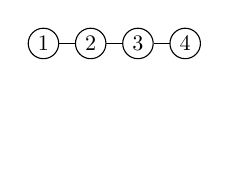
\begin{tikzpicture}[scale=0.6, every node/.style={scale=0.8,inner sep=.7mm}]
          \node [draw,circle] (1) at (0,0) {1};
          \node [draw,circle] (2) at (1,0) {2};
          \node [draw,circle] (3) at (2,0) {3};
          \node [draw,circle] (4) at (3,0) {4};
	  \node[] () at (0,-2.5) {};   % just to move the picture up a bit
          \draw (1) -- (2);
          \draw (2) -- (3);
          \draw (3) -- (4);
        \end{tikzpicture}
        \label{fig:assoc-g}
    }
    \quad\subfigure[][$H$] {
        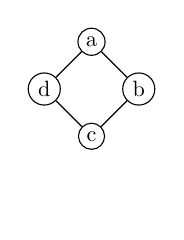
\begin{tikzpicture}[scale=0.6, every node/.style={scale=0.8,inner sep=.7mm}]
          \node [draw,circle] (a) at (1,2) {a};
          \node [draw,circle] (b) at (2,1) {b};
          \node [draw,circle] (c) at (1,0) {c};
          \node [draw,circle] (d) at (0,1) {d};
	  \node[] () at (0,-1.5) {};   % just to move the picture up a bit
          \draw (a) -- (b);
          \draw (b) -- (c);
          \draw (c) -- (d);
          \draw (d) -- (a);
        \end{tikzpicture}
        \label{fig:assoc-h}
    }
    \quad\subfigure[][Association graph] {
        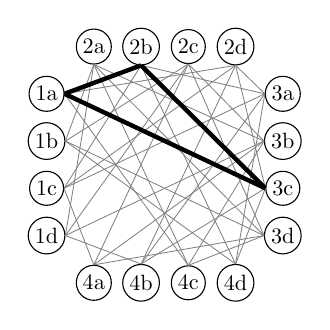
\begin{tikzpicture}[scale=0.6, every node/.style={scale=0.8,inner sep=.5mm}]
          \node [draw,circle] (1a) at (0,4) {1a};
          \node [draw,circle] (1b) at (0,3) {1b};
          \node [draw,circle] (1c) at (0,2) {1c};
          \node [draw,circle] (1d) at (0,1) {1d};
          \node [draw,circle] (2a) at (1,5) {2a};
          \node [draw,circle] (2b) at (2,5) {2b};
          \node [draw,circle] (2c) at (3,5) {2c};
          \node [draw,circle] (2d) at (4,5) {2d};
          \node [draw,circle] (3a) at (5,4) {3a};
          \node [draw,circle] (3b) at (5,3) {3b};
          \node [draw,circle] (3c) at (5,2) {3c};
          \node [draw,circle] (3d) at (5,1) {3d};
          \node [draw,circle] (4a) at (1,0) {4a};
          \node [draw,circle] (4b) at (2,0) {4b};
          \node [draw,circle] (4c) at (3,0) {4c};
          \node [draw,circle] (4d) at (4,0) {4d};
	  \draw[color=gray, line width=.3] (1a.east) -- (2d.south);
\draw[color=gray, line width=.3] (1a.east) -- (4c.north);
\draw[color=gray, line width=.3] (1b.east) -- (2a.south);
\draw[color=gray, line width=.3] (1b.east) -- (2c.south);
\draw[color=gray, line width=.3] (1b.east) -- (3d.west);
\draw[color=gray, line width=.3] (1b.east) -- (4d.north);
\draw[color=gray, line width=.3] (1c.east) -- (2b.south);
\draw[color=gray, line width=.3] (1c.east) -- (2d.south);
\draw[color=gray, line width=.3] (1c.east) -- (3a.west);
\draw[color=gray, line width=.3] (1c.east) -- (4a.north);
\draw[color=gray, line width=.3] (1d.east) -- (2a.south);
\draw[color=gray, line width=.3] (1d.east) -- (2c.south);
\draw[color=gray, line width=.3] (1d.east) -- (3b.west);
\draw[color=gray, line width=.3] (1d.east) -- (4b.north);
\draw[color=gray, line width=.3] (2a.south) -- (3b.west);
\draw[color=gray, line width=.3] (2a.south) -- (3d.west);
\draw[color=gray, line width=.3] (2a.south) -- (4c.north);
\draw[color=gray, line width=.3] (2b.south) -- (3a.west);
\draw[color=gray, line width=.3] (2b.south) -- (4d.north);
\draw[color=gray, line width=.3] (2c.south) -- (3b.west);
\draw[color=gray, line width=.3] (2c.south) -- (3d.west);
\draw[color=gray, line width=.3] (2c.south) -- (4a.north);
\draw[color=gray, line width=.3] (2d.south) -- (3a.west);
\draw[color=gray, line width=.3] (2d.south) -- (3c.west);
\draw[color=gray, line width=.3] (2d.south) -- (4b.north);
\draw[color=gray, line width=.3] (3a.west) -- (4b.north);
\draw[color=gray, line width=.3] (3a.west) -- (4d.north);
\draw[color=gray, line width=.3] (3b.west) -- (4a.north);
\draw[color=gray, line width=.3] (3b.west) -- (4c.north);
\draw[color=gray, line width=.3] (3c.west) -- (4b.north);
\draw[color=gray, line width=.3] (3c.west) -- (4d.north);
\draw[color=gray, line width=.3] (3d.west) -- (4a.north);
\draw[color=gray, line width=.3] (3d.west) -- (4c.north);
\draw[ultra thick] (1a.east) -- (2b.south);
\draw[ultra thick] (1a.east) -- (3c.west);
\draw[ultra thick] (2b.south) -- (3c.west);

        \end{tikzpicture}
        \label{fig:assoc}
    }
    \caption{Two graphs and their association graph.  The edges of a maximum
    clique in the association graph are highlighted. This corresponds to a maximum
    common induced subgraph: the subgraph of $G$ induced by $\{1,2,3\}$,
    which is isomorphic to the subgraph of $H$ induced by $\{a,b,c\}$.}
    \label{fig:intro-assoc-graph}
\end{figure}

\citet{durand1999efficient}

The RASCAL algorithm \citep{raymond2002rascal} solves MCES by finding a maximum
clique in the modular product graph of the line graphs.  The algorithm is
optimised for matching chemical structures, and does not solve the maximum common
\emph{connected} subgraph problem.  In addition to greedy
colouring, the algorithm uses a number of other heuristic colourings to derive
an upper bound depending on the size of the modular product graph.  Unfortunately
the authors were unable to provide code for RASCAL.

\cite{DBLP:conf/cp/McCreeshNPS16} uses a state of the art maximum clique algorithm
to solve this problem, and introduces a modified version of the algorithm to
solve maximum common \emph{connected} induced subgraph.

\subsection{Constraint programming algorithms}

\citet{DBLP:journals/spe/McGregor82}
introduced a branch and bound algorithm for the maximum common
\emph{edge} subgraph problem in which a vertex of $G$ is mapped to a vertex
of $H$ at each node of the search tree.  A matrix of boolean values indicates
the set of edges in $H$ to which each edge in $G$ may be mapped; this may be
viewed as a simple domain store. \citet{DBLP:conf/sspr/BunkeFGSV02}
reports using McGregor's algorithm to solve MCIS, without giving full
details of the modifications made to the algorithm.

\citet{DBLP:conf/mco/VismaraV08} give a constraint model for solving maximum
common connected edge subgraph based on solving MCIS on the line graphs of the
two input graphs; effectively, this is the first formal constraint program for
MCIS.  Like the CP model for induced subgraph isomorphism in
\Cref{subsec:cp-model-isip}, we have a variable $x_v$ for each $v \in V(G)$.
Each domain is $V(H) \cup \bot$, where $\bot$ is special value indicating that
a vertex is unmapped.  The objective is to minimise the number of $\bot$
values.  The model uses binary constraints to ensure that no two vertices in
$G$ are mapped to the same vertex in $H$.  The adjacency and non-adjacency
constraints from our induced subgraph isomorphism model are replaced by the
following, in order to allow any vertex to be mapped to $\bot$.

\begin{itemize}
    \item For all distinct $v, w \in V(G)$ such that $v \in N_G(w)$, we have 
$x_v=\bot$,
$x_w=\bot$, or
$x_v \in N_H(x_w)$.
\item For all distinct $v, w \in V(G)$ such that $v \not\in N_G(w)$, we have 
$x_v=\bot$,
$x_w=\bot$, or
$x_v \not\in N_H(x_w)$.
\end{itemize}

\citet{DBLP:conf/cp/NdiayeS11} present a CP model that shares the variables
of the \citeauthor{DBLP:conf/mco/VismaraV08} model, but replaces the binary difference
constraints with a single global ``soft allDiff''
constraint \citep{DBLP:conf/cp/PetitRB01}.  This ensures that distinct vertices
in $G$ are mapped to distinct vertices in $H$, and uses a matching algorithm
to calculate a stronger upper bound than the one given by
the \citeauthor{DBLP:conf/mco/VismaraV08} model.
\citeauthor{DBLP:conf/cp/NdiayeS11} carry out detailed experiments using
different levels of consistency for the adjacency and soft allDiff constraints.
The soft allDiff constraint, which used to calculate an upper bound but
not to filter domains, causes the algorithm to run several times faster
than the simple difference constraints used by \citeauthor{DBLP:conf/mco/VismaraV08}.
Comparing forward checking (FC) and maintaining arc consistency (MAC)
on the adjacency constraints, FC outperforms MAC on unlabelled instances
while MAC outperforms FC on labelled instances.

\cite{DBLP:conf/cp/McCreeshNPS16} add a connectedness constraint to
the CP model of \citet{DBLP:conf/cp/NdiayeS11}.  This is found to perform
better overall than simply branching on vertices adjacent to some already-mapped
vertex in order to ensure connectedness.

\subsection{Subgraph enumeration algorithms}

Finally, we mention briefly a very different technique that has been used
in a number of papers to find a maximum common connected subgraph between two or more
graphs representing molecules.
\citep{armitage1967automatic}
\citep{takahashi1987recognition}
\citep{DBLP:journals/jcheminf/DalkeH13}
In this type of algorithm, connected
subgraphs of the first graph are built one node at a time by a tree search.
A subgraph isomorphism solver is used to test whether each of these subgraphs
appears in each of the other input graphs.  In some versions of this algorithms,
the subgraphs of $G$ are tested for isomorphism with previously-generated subgraphs
in order to break symmetries.
Unfortunately, we have been unable to find an implementation of this technique
for MCIS in general graphs to use in our experimental evaluation.

\subsection{Misc stuff to sort out}

\citet{cao2008maximum} is a backtracking algorithm that does not store domains,
but tests before making each assignment $(v,w)$ whether the set of vertices in $M$
that are adjacent to $v$ in $G$ corresponds to the set of vertices in $M$ that
are adjacent to $w$ in $H$.  The main upper bound proposed by the authors
is, in CP terms, the bound given by adding to $|M|$ the number of unassigned
variables whose domains contain at least one vertex.  The authors also outline
a matching upper bound.  In each case, it appears likely that the fact that the algorithm does not
store domains results in substantial addition work on each call of the upper bound
function.  (TODO tidy up that last sentence!)

\citet{DBLP:conf/cp/McCreeshNPS16} TODO talk about clique algo, new version
of clique algo for connected. TODO check: do they introduce a new connected
constraint? Do I compare against this in McSplit chapter?

\section{New algorithms in this thesis}

The McSplit family of algorithms has branch-and-bound variants and variants
that use a sequence of decision problems; it also has variants for induced and
edge subgraph problems. The summary in this section discusses only the induced
variants.

McSplit performs tree search in the style of a forward-checking constraint
programming algorithm. Rather than maintaining an explicit domain for each
vertex in the first graph, vertices are re-labelled at each search node in such
a way that the current mapping may only be extended by mapping a vertex in
first graph to a vertex in the second graph with the same label. Labels may be
viewed as equivalence classes of vertices, and at each search node these
classes are refined (partitioned) into smaller classes. We store the vertices
of each graph as a list (without copying at each search node), and can perform
this partitioning efficiently be re-arranging the vertices in each list. This
data structure makes it possible to calculate an upper bound very cheaply at
each search node, and permits the cheap computation of good variable-ordering
heuristics.

\section{Experimental setup}

The experiment in chapters ... were run on ...

The experiments in chapter ... were run on ...

All solvers were compiled using GCC version 9.4.0 with the flags
\texttt{-O3} (optimization level 3) and \texttt{-march=native}
(which allows the compiler to use any CPU instruction that is available
on the machine, and is particularly helpful in improving the performance
of the Glasgow Subgraph Solver).

\section{Conventions for Plots}

Scatter plots and cumulative plots are used frequently in this dissertation to
compare the run times of algorithms.  To illustrate how these will be used,
consider the run times in milliseconds for ten hypothethetical instances,
with one row per instance, in \Cref{fig:intro-dummy-table}.

\Cref{fig:intro-dummy-scatter} shows a scatter plot of these run times. Log
scales are used for run times throughout this dissertation. Since run times are
measured at a 1 millisecond resolution, the points are jittered by adding a
uniform random number in the range $[-1/2,1/2)$ to each time. This reduces
over-plotting and thus helps to show the distribution of points, with only a
negligible effect on the plots' precision. Run times of zero are ploted in the
range $[1/2,1)$ because zero cannot appear on a log scale.  Timeouts (exceeding
1000 seconds) appear in the grey band just beyond a run time of 1000 seconds;
again, we jitter these within the band to minimise over-plotting. The line
$x=y$, where the two algorithms have the same run time, is show for
convenience.

\Cref{fig:intro-dummy-cumu} shows a less common type of figure: an
\emph{empirical cumulative distribution function plot} (henceforth
\emph{cumulative plot}). For a given run time $t$ (on the horizontal axis),
this answers the question ``how many of the instances can be solved in less
than $t$ milliseconds per instance?'' Equivalently, it answers the question
``if the per-instance time limit were reduced to $t$, how many instances would
each algorithm solve?''
We can see, for example, that Algorithm A can solve six
of the instances within 10 ms (the first six instances in the table),
while Algorithm B can solve only three instances
within that time.

\begin{figure}[htb]
    \centering
    \subfigure[][Hypothetical run times per instance] {
        \tiny
        \includegraphics*[width=0.2\textwidth]{10-introduction/plot-examples/table/table}
        \label{fig:intro-dummy-table}
    }
    \subfigure[][Scatter plot of run times] {
        \includegraphics*[width=0.39\textwidth]{10-introduction/plot-examples/plots/scatter}
        \label{fig:intro-dummy-scatter}
    }
    \subfigure[][Cumulative plot of run times] {
        \includegraphics*[width=0.34\textwidth]{10-introduction/plot-examples/plots/cumulative}
        \label{fig:intro-dummy-cumu}
    }
    \caption{Hypothetical run times in ms for two solvers on ten instances: table,
        scatter plot, and cumulative plot. The time limit is 1000 seconds.}
    \label{fig:intro-dummy-figs}
\end{figure}

\section{Structure of the Dissertation}

The remainder of this dissertation is structured as follows.

\paragraph*{\ChapterRef{c:mcsplit-i-undirected}} introduces the \McSplit\ algorithm
for the maximum common induced subgraph problem and its variants, and carries out
an experimental comparison with existing state of the art solvers.

\paragraph*{\ChapterRef{c:swapping-graphs-mcsplit}} asks whether and when
it is useful to swap the two graphs given as input to a \McSplit.  We develop
two simple rules for determining when to swap the graphs, and generalise
these to the algorithm \McSplit-2S which branches on vertices of both
input graphs.

\paragraph*{\ChapterRef{c:mcsplit-si}} introduces the \McSplit-SI algorithm for the
induced subgraph isomorphism problem.  This is based on \McSplit, but uses
special data structures designed to work well if the input graphs are sparse.
We present an extensive set of experiments comparing the algorithm to state of
the art solvers.  Finally, we modify \McSplit-SI to solve the maximum common
induced subgraph problem, and show that it outperforms the state of the art
solver for large, sparse graphs.

\paragraph*{\ChapterRef{c:mcsplit-i-undirected}} introduces exact and heuristics
for the minimum induced universal graph problem.

\paragraph*{\ChapterRef{c:conclusion}} concludes.

\section{Miscellaneous notes}

MCIS is NP-hard, even if graphs are both bipartite.  This can be shown by a
reduction from maximum induced matching.  (I think the proof for maximum induced
matchings is in Induced Matchings (1989) by Kathie Cameron). Is there another
proof somewhere?

Independent set is NP-hard on planar graphs (see Wikipedia).  Therefore
MCIS also is.

Cuissart and Hebrard 2005 A Direct Algorithm to Find a Largest Common
Connected Induced Subgraph of Two Graphs doesn't seem to do any
pruning.  Is it slow?

\section{Publications}

During the course of my PhD I carried out further work
that is not presented in this thesis.
For completeness, the following is a full list of publications
since the start of my PhD.  The first of these
forms the basis of \Cref{c:mcsplit-i-undirected}.

\begin{itemize}
    \item\bibentry{DBLP:conf/ijcai/McCreeshPT17}
    \item\bibentry{DBLP:conf/cp/McCreeshPST17}
    \item\bibentry{DBLP:conf/cpaior/HoffmannMNPRS018}
    \item\bibentry{DBLP:journals/jair/McCreeshPST18}
    \item\bibentry{DBLP:conf/cpaior/ArchibaldDHMP019}
    \item\bibentry{DBLP:conf/wea/000120a}
    \item\bibentry{DBLP:conf/iwpec/000120}
    \item\bibentry{DBLP:conf/iwpec/000120a}
    \item\bibentry{DBLP:conf/gg/McCreeshP020}
    \item\bibentry{DBLP:conf/cp/GochtMMNPT20}
    \item\bibentry{DBLP:journals/cor/DelormeGGKMPT22}
\end{itemize}

%==============================================================================
\section{Thesis Statement}
\label{c:intro:thesisstatement}

TODO

